\documentclass[../book.tex]{subfiles}

\chapter{Regularizing and materializing objects}
\label{ch:genome}

\begin{quote}
Science is concentrated in an area of knowledge it does not absorb and
in a formation which is in itself the object of knowledge and not of
science.\autocite[19]{Deleuze_1988}
\index{Deleuze, Gilles!knowledge and science}
\end{quote}

What is the materiality of machine learning?
\index{machine learning!materiality|see{materiality}} The opening pages
of \emph{Elements of Statistical Learning} present four somewhat
excessive objects -- spam email, handwritten digits, prostate cancer,
and `DNA Expression Microarrays' -- and list six examples (document
classification, image recognition, risk of heart attack, stock price
prediction, risk factors for prostate cancer, and glucose estimates for
diabetics) \autocite[1-7]{Hastie_2009}. What happens to things like
prostate cancer, handwritten digits or stock prices when machine
learners ply them? Although machine learning occurs in the thick of a
control crisis \autocite{Beniger_1986}\index{control!crisis of} (as
suggested in chapter \ref{ch:introduction}), I will suggest here machine
learning also occasions viscous multi-temporal and inter-objectively
distributed enactments of things such as financial markets, media
platforms, chronic diseases and living things. These are all
hyperobjects \index{hyperobject} that epistemically, infrastructurally,
economically and socially individuate through machine learning.

The last of the vignettes, the DNA microarray, comes from the life
sciences. It attracts a whole page colour figure -- a
heatmap.\autocite[7]{Hastie_2009}\footnote{I have discussed the history
  of heatmaps and their place in contemporary science in other work
  \autocite{Mackenzie_2013c}.} \index{data!DNA microarray}.
\index{graphic!heatmap} DNA, genes, genomics and proteomics then more or
less disappear from view for the next 503 hundred pages of the book
(aside from a brief mention in the context of cross-validation), only to
abruptly reappear in a discussion of unsupervised machine learning
techniques (k-means, agglomerative and hierarchical clustering; Chapter
14, where the DNA microarray data is re-analysed using hierarchical
clustering\index{machine learner!hierarchical clustering}), and then
again, and much more extensively, in a final chapter (Chapter 18) new to
the second edition of the book on `High Dimensional Problems.' Apart
from one passage where the Hastie and co-authors develop a document
classifier for their own journal articles, every example in the added
Chapter 18 comes from genomic science, a scientific field that largely
begins to take a recognisable shape in the late 1990s as both sequence
data and high-throughput DNA-analysis devices, particularly microarrays,
become widely available. \index{genomics!importance in machine learning}

Operational formations usually encompass scientific fields. Alongside
the operational problems of spam email filtering, image or handwriting
recognition, scientific research into biological processes constitutes a
major reference point and, I will suggest, an axis of materialisation
for machine learning. In the archaeology of its operational formation,
we could say that the scientific domain of genomics has a strongly
referential effect on machine learning. What is a \gls{referential}? For
Foucault, a referential `forms the place, the condition, the field of
emergence, the authority to differentiate between individuals or
objects, states of things and relations that are brought into play by
the statement itself; it defines the possibilities of appearance and
delimitation of that which gives meaning to the sentence, a value as
truth to the proposition' \autocite[91]{Foucault_1992}.
\index{referential!entanglement} For Foucault, a referential forms an
integral part of the enunciative function, the mapping of sites, subject
positions, enunciative modalities, forms of accumulation and
differentiation at work in the production of statements.
\index{statements!referential of}

Why does the referential of machine learning matter? When hyperobjects
are machine learned, they are re-constituted (in vector space, as
optimisation problems, as probability distributions and patterns of
difference). Conversely, as I will suggest in this chapter, they become
a site of materialization, cross-validation and regularization for
machine learning in its production of knowledge. But that referential
status, which authorises and imbues statements with value, comes at a
cost. The plurality or multiplicity of the hyperobject -- genomes, stock
prices, etc. -- will be regularized and ranked, re-used and transcribed
by machine learners over and over to lend coherence to the operational
formation and its system of statements.

\section{Genomic referentiality and
materiality}\label{genomic-referentiality-and-materiality}

\begin{quote}
\texttt{gaagctccac\ accagccatt\ acaaccctgc\ caatctcaag\ cacctgcctc\ tacaggtacc}
\autocite{NCBI_2016}
\end{quote}

By contrast with industry, commerce, media and government, where much
that happens is obscured from view, the great virtue or genomic science
is the relative openness of its workings and its resolute insistence on
DNA as the primary form of data. The fact that data practices are
relatively generic and accessible means that critical research into
transformations associated with genomic data and knowledge can accompany
nearly every aspect of practice. \index{science!genomics!openness of}

Genomic data exhibits some specific features. The first concerns what I
earlier called data strain. \index{data!strain} Genome data, a tiny
fragment of which is shown above, inflates the vector space. Genomics
generates new versions of the now familiar problems of data
dimensionality. The abundance, diffusion, heterogeneity or impaction of
genomic data thwarts its examination, tabulation, and regulated
circulation. Genomics data also presents unusual ratios of accumulation
and sparsity. Clinical genomics in particular generates datasets that
are lavishly furnished with `features' but often quite meagrely supplied
with clinical cases or `observations'. In the shorthand typical of
machine learning terminology, \(p\) is larger than \(N\): `the number of
features \(p\) is much larger than the number of observations \(N\),
often written \(p\gg N\)' \autocite[649]{Hastie_2009}. This strains
statistical methods that rely on the \(\forall{\boldsymbol{X}}\) `Law of
Large Numbers' \autocite[99-104]{Hacking_1990}, which holds that the
accuracy of statistics tends to increase with more observations.
\index{statistics!Law of Large Numbers}

Since the early nineteenth century, biology and cognate disciplines have
sought to explore problems of time, genesis, duration, activity and
process in a very broad spectrum of living things. Contemporary genomics
seeks to elicit, as many commentators have noted, knowledge of
biological, evolutionary, biomedical and environmental processes from
the long DNA sequences comprising genomes. The primary `object' in
genomics is a \(\forall{\boldsymbol{X}}\) data form, the genome, the
full complement of DNA in an organism.\index{data!all of} Genomes vary
in size from the 2000 DNA base pairs of a virus, the 3.2 Gb (gigabase
pairs) of humans through to the 130 Gb of the lung fish. The founding
premise of genomic science is that a dataset comprising the complete
sequence of DNA potentially re-bases knowledge of many different
biological processes, ranging from evolution (phylogeny), development
(ontogeny), metabolism, structure and pathology.
\index{function!biological} If nothing else, genome comparison promises
knowledge of the 3.8 billion years of evolution of species differences
and population diversity. \index{differences!species} In all of these
respects, DNA sequences have since at least the 1980s served as the
common substrate for many different scientific experiments, technical
developments, cyber-infrastructures and needless to say, biological
imaginaries oriented around the problems of control.\footnote{A large
  and very diverse social science and humanities literature now exists
  around genomics. I draw on some of that literature as general
  background here, especially
  \autocites{SunderRajan_2006}{Thacker_2005a}{Stevens_2011}{Leonelli_2014}
  and \autocite{Haraway_1997}, but largely do not address it directly.}

The genomic premise has an ineluctably promissory association with
knowledge economy. \index{knowledge!totality of} Prior to the whole
genome sequencing projects initiated in the 1990s, biologists had never
worked with genomes only with selected DNA sequences, especially those
associated with genes and the proteins that they code. By contrast, the
genome, with all its repeated, redundant, and slightly varying patterns
of DNA, bears the traces of long evolutionary mixing and constitutes a
hyper-complex functional process whose exquisite sensitivity to changing
conditions -- a slight change in light reaching a leaf cascades can be
traced in patterns of DNA transcription -- forms an extreme case for any
operational sense of function. The functioning of genomes symbolises a
deeply interconnected relationality in life sciences, and becomes the
test case for the learning capacities of machine learners.\footnote{As
  data forms, genomes have a problematic mode of existence. They
  resemble cat images on the internet. As a data form, genomes are
  remarkably homogeneous. They are one-dimensional strings of letters
  corresponding to the well-known four nucleic acids (\texttt{g},
  \texttt{a}, \texttt{t}, \texttt{c}). \index{data!form of!genomic}
  While many earlier tabulations of variation, difference, groups, types
  and relations are woven through the life sciences, genomes have for
  the last several decades mesmerised biological sciences as a way of
  analysing and re-distributing the confused multiplicities associated
  with living things. The raw data for genomes comes from the sequencing
  of DNA obtained from various organisms - viruses, bacteria, plants,
  fish, animals and humans. The sequencing of DNA, especially DNA that
  encodes the proteins that pervade biological processes, that structure
  tissues or assemble in complicated metabolic pathways, has been the
  concern first of molecular biology (mainly in the 1970s-1990s) and
  more recently genomics (post-1990). In molecular biology, DNA
  sequences were carefully elicited (using the experimental techniques
  for instance of Sanger sequencing) and then compared with already
  known sequences of DNA to identify similarities that might have
  biology significance (for instance, evolution from a common ancestor).
  In genomics, DNA sequences generally originate from increasingly
  high-throughput sequencers that output massive datasets (see
  \autocites{Stevens_2013}{Mackenzie_2015}. Given both the accumulated
  store of already sequenced DNA and the increasingly viable practices
  of sequencing all of the DNA in a given organism, genomics has
  promised a much wider and more detailed understanding of biological
  complexity than any previous life science had been able to obtain.
  With genomes in hand, biologists for the first time would be in a
  position to build models of entire domains of biology, domains that
  previously could only be explored through painstaking experiments
  targeting specific cells, molecules, biochemical reactions and
  networks. The vast yet somewhat dispersed knowledges of the life
  sciences might be re-ordered and aligned on a new very extensive yet
  quite homogeneous backbone of the genome read out as billions of DNA
  base pairs.} \index{science!genomics!premise and promise of}

As referentials, genomes pose a problem of unregulated abundance and
seeming homogeneity. DNA sequences exist in great abundance (in
databases, and increasingly, from the cheaper and more compact
sequencing instruments), yet even determining how DNA sequence fragments
should be ordered in a genome -- let alone how they make sense as some
biological function -- is much harder. DNA sequences are assembled as
genomes and genomic datasets via statistical models.
\index{data!assembly} \index{data!sequence!DNA} `Genome assembly
continues to be one of the central problems of bioinformatics' write the
authors of a recent scientific review of the techniques of constructing
whole genomes from DNA sequencer data \autocite{Henson_2012}. Even the
elementary data form of the genome as DNA base pairs is a highly
algorithmic construct. No existing sequencing technology produces a
genome as a single sequence, as a vector (in the sense described in
chapter \ref{ch:vector}). Instead, sequencing produces random sets of
sequence fragments of various lengths that have to be assembled into a
complete genome algorithmically. \footnote{Whole genome assembly as
  reported for the initial draft of the human genome in 2001
  \autocites{Venter_2001}{Lander_2001} or for the model biological
  organism, \emph{Drosophila} \autocite{Myers_2000} was not at the time
  understood as a machine learning problem. The task of whole genome
  assembly from DNA fragments was seen as probabilistic in the sense
  that the aim is to assemble the often millions of short sequence
  fragments in an order that is most likely to occur. Even prior to the
  first full human genome assembly, genomic science had made heavy use
  of probabilistic models in aligning DNA (and protein amino acid)
  sequences. Richard Durbin, Sean Eddy, Anders Krogh and Graeme
  Mitchison's highly cited \emph{Biological Sequence Analysis:
  Probabilistic Models of Proteins and Nucleic Acids}
  \autocite{Durbin_1998} was based almost entirely on Hidden Markov
  Models, a way of modelling a sequence of states that \emph{Elements of
  Statistical Learning} treats at chapter length (see \autocite[Chapter
  17]{Hastie_2009}).
  \index{machine learner!Hidden Markov Model!in genome assembly} While
  sequence alignment was regarded as a deeply algorithmic and
  statistical problem in the former volume, it is not at all formulated
  in the language of machine learning. There is little discussion of
  cost functions, vector spaces, optimisation, problems of
  generalization, supervised or unsupervised learning. On the other,
  David Haussler, a key bioinformatician in the first draft of the human
  genome in his work explicitly sought to bring machine learning methods
  to bear on biology, and continues to do so. See
  \autocite{Zerbino_2012} for a review of the relevance of machine
  learning to genomic science. The practical problem here is that
  genomes contain swathes of duplicated regions that make assembling
  sequences in good order a severe challenge. While sequence alignment
  algorithms have long used algorithmic approaches (known as dynamic
  programming) to score the similarity between two given DNA sequences,
  assembling the millions of DNA sequences produced by contemporary
  sequencers has necessitated entirely new techniques (shifting, for
  instance, from the overlap-layout-consensus model to the de Bruijn
  graph-based path models \autocite{Pevzner_2001}.
  \index{machine learner!Hidden Markov Model} \index{Haussler, David}}

Between pre-genomic and post-genomic science, the status of significant
differences in genomes shifted. \index{differences!variation as} Pre-HGP
biology understood the significant differences between individual
organisms largely in terms of gene alleles responsible for variations in
phenotypes. Biological differences, and disease in particular, stemmed
from different forms of genes. Understanding disease meant finding the
disease genes. Even prominent proponents of genomics, such as Leroy
Hood, writing of `Biology and Medicine in the Twenty-First Century' in
1991, envisaged genomics as a way of simplifying `the task of finding
disease genes' \autocite[138]{Hood_1992}. Across the life sciences,
genes were the object of much way of annotation, labelling and
description. Two decades after the inception of whole genome sequencing,
genomes present a different image of variation. According to Nikolas
Rose, writing more recently, `there is no normal human genome; variation
is the norm' \autocite[75]{Rose_2009}.
\index{Rose, Nikolas!on normal variation} \index{genome!variation in}
`In this new configuration', he writes, `what is required is not a
binary judgment of normality and pathology, but a constant modulation of
the relations between biology and forms of life, in the light of genomic
knowledge.' The emphasis in Rose' formulation falls on `constant
modulation' of the relations between biology and forms of life. If
post-genomic science departs from the understanding that there is no
single genome but many genomes, then according to Rose, variation itself
becomes of primary interest. Pursuit of variation remakes the genome
into `a form whose only object is the inseparability of distinct
variations' \autocite[21]{Deleuze_1994}.
\index{hyperobject!variation in}

Whatever knowledge subsequently derives from a genome (genes, mutations,
evolutionary relationships, variations associated with disease, heredity
or individual identity), genomic data and hence the genome itself as a
scientific hyperobject \index{hyperobject!genome as} is deeply
probabilistic. From assembly onwards, through the ancestral
probabilisation embodied in heavily-used biological databases, the
indelible errors, the entangled reliances on accumulated biological
knowledges make genomes a particularly challenging site of machine
learning activity.

\emph{Elements of Statistical Learning}'s invocation of DNA-related
data, therefore, is no arbitrarily chosen example amidst the general
proliferation of settings, domains, cases and examples typically found
in machine learning pedagogy. In multiple dimensions and directions,
genomics -- the scientific project of operating on the whole DNA
complement of organisms -- is a tightly coupled referential for machine
learning even if relatively few machine learners have, to date, managed
to work with whole genome sequence data. The relatively long-established
referential entanglement (at least 25 years, and perhaps more) of
genomics and machine learning is strategically important in the
generalization of machine learning, in the processes whereby techniques,
with their specific forms of articulation, statement and making-visible,
propagate into multiple, once-disparate settings.\footnote{Signal
  processing is another such domain. Many of the techniques now
  prominent in machine learning developed in parallel in signal
  processing, where the encoding and decoding of signals has long been
  seen as a problem of pattern recognition amenable to statistical
  calculation. In some specific cases, such as Hidden Markov Models, the
  same techniques seem to appear almost simultaneously in very disparate
  domains. Hidden Markov Models appear in genomics (as part of the
  problem of sequence alignment) at the same time as the begin to appear
  in digital signal processing for wireless communication and video
  image compression \autocite{Mackenzie_2010a} and above all, in speech
  recognition \autocite{Rabiner_1989}.
  \index{signal processing!relation to machine learning}
  \index{machine learner!Hidden Markov Model}}
\index{diagram!diagrammatization!as generalization} Like social media
platforms or retail spaces with their many visitors, genomes, I would
suggest, provoke a multiplicity of machine learners to bind to them like
antibodies to an antigen (or an allergen). Genomes function as
regularizing hyperobjects for machine learning.
\index{machine learning!regularizing hyperobjects}

\section{The genome as threshold
object}\label{the-genome-as-threshold-object}

\begin{table}[ht]
\centering
\begingroup\tiny
\begin{tabular}{p{0.1\textwidth}p{0.1\textwidth}p{0.8\textwidth}}
  \hline
 & Frequency & Discipline \\ 
  \hline
1 & 1302 & computer science, artificial intelligence \\ 
  2 & 924 & engineering, electrical \& electronic \\ 
  3 & 520 & statistics \& probability \\ 
  4 & 401 & computer science, information systems \\ 
  5 & 344 & computer science, interdisciplinary applications \\ 
  6 & 332 & biochemistry \& molecular biology \\ 
  7 & 281 & mathematical \& computational biology \\ 
  8 & 259 & biotechnology \& applied microbiology \\ 
  9 & 257 & biochemical research methods \\ 
  10 & 228 & neurosciences \\ 
  11 & 218 & computer science, theory \& methods \\ 
  12 & 199 & radiology, nuclear medicine \& medical imaging \\ 
  13 & 198 & multidisciplinary sciences \\ 
  14 & 189 & genetics \& heredity \\ 
  15 & 181 & immunology \\ 
  16 & 157 & ecology \\ 
  17 & 155 & imaging science \& photographic technology \\ 
  18 & 125 & automation \& control systems \\ 
  19 & 122 & engineering, biomedical \\ 
  20 & 106 & computer science, hardware \& architecture \\ 
   \hline
\end{tabular}
\endgroup
\caption{The top 20 disciplines of the top 5000 cited research publications in machine learning, 1990-2015} 
\label{tab:top_discp}
\end{table}

During 1990-2015, biology, and particularly molecular and then genomic
biology, has a very high visibility in the machine learning research
literature. (See table \ref{tab:top_discp}.) After the leading machine
learning disciplines (computer science, electronic engineering and
statistics), molecular biology, genomics and bioinformatics attract most
academic journal citations and publications associated with machine
learning. Half of the most cited research literature has a biomedical or
life science referentiality. This may be because genomes and human
disease in particular, are premiere scientific hyperobjects like the
human brain, dark matter, global climate or fundamental particles in
contemporary sciences. \index{hyperobject} \index{genome!as hyperobject}
But it might also be the case -- and I will pursue this line of argument
here -- that genomes, with all their operational and functional
complexity, come into play, are potentialized and regulated, and take on
promissory epistemic value as zones of collective individuation through
machine learning. In terms of contemporary biological knowledge
production, the transformation of biology into a data-intensive science
\autocites{Hey_2009}{McNally_2012} is tightly entangled with machine
learning in processes of cross-validation.
\index{genomics!as cross-validation of machine learning}

In the generalization of machine learning, the genomic referential marks
a threshold of materialization. \index{referential! threshold of}
\index{materiality!as infrastructure} The archaeological approach to
materiality is somewhat unusual. Given his interest in the formation of
statements, Foucault understands materiality as a regulatory process
operating in an enunciative function. Foucault writes:

\begin{quote}
The rule of materiality that statements necessarily obey is therefore of
the order of the institution rather than of the spatio-temporal
localization; it defines possibilities of reinscription and
transcription (but also thresholds and limits) , rather than limited and
perishable individualities \autocite[103]{Foucault_1972}
\index{Foucault, Michel!on statements!materiality of}
\end{quote}

In the archaeology of an operational formation, locating specific
practices, places and times of reinscription, transcription, and
possibilities of reuse carries more weight more than any direct
conceptual account of materiality. \index{archaeology!materiality in}
What would materiality in this sense mean for machine learning?

Genomes are both a challenge to the capacity of machine learning to
produce scientific knowledge \index{knowledge!scientific} (as distinct
from say the unstable commercial knowledge of a credit risk model), and
a cross-validation of machine learning as a life-death relevant
knowledge practice. Genomes first of all authorize infrastructural
vectorizations such as computational clusters, grids, arrays and clouds.
\index{vectorization!infrastructural} For instance, the Google Compute
Engine, a globally addressable ensemble of computers typical of recent
distributed commercial computing architectures, was briefly turned over
to exploration of cancer genomics during 2012, and publicly demonstrated
at the annual Google I/O conference. \index{Google!I/O Conference, 2012}
Midway through the demonstration, in which a human genome is visualized
as a ring in `Circos' form (see figure \ref{fig:circos}
\autocite{Krzywinski_2009}), the speaker, Urs Hölzle, Senior Vice
President of Infrastructure at Google `then went even further and scaled
the application to run on 600,000 cores across Google's global data
centers' \autocite{GoogleInc.2012}. \index{Google!Google Compute Engine}
The audience clapped as the annular diagram of a human genome was
decorated with a rapidly increasing number of cross-links, accompanied
by a snapping sound as it appeared. The world's `3rd largest
supercomputer', as it was called by \emph{TechCrunch}, a prominent
technology blog, `learns associations between genomic features'
\autocite{Anthony_2012}. Note the language of machine learning: it
`learns \ldots{} associations between features.' We are in the midst of
many such demonstrations of `scaling applications' of data in the
pursuit of associations between `features.'\footnote{A second
  significant and equally prestigious example of this infrastructural
  re-scaling might be IBM Corporation's `cognitive computing platform,'
  Watson. Watson, a distributed computing platform centred on machine
  learning, is hard to delineate or easily describe since it exists in a
  seemingly highly variable form. Its uses in genomics, pharmaceutical
  discovery, clinical trials and cooking are heavily promoted by IBM
  \autocite{IBM_2014}. Another would be Amazon Web Services various
  cloud computing services, some of which have been heavily used by
  genomic scientists.}

\begin{figure}
  \centering
      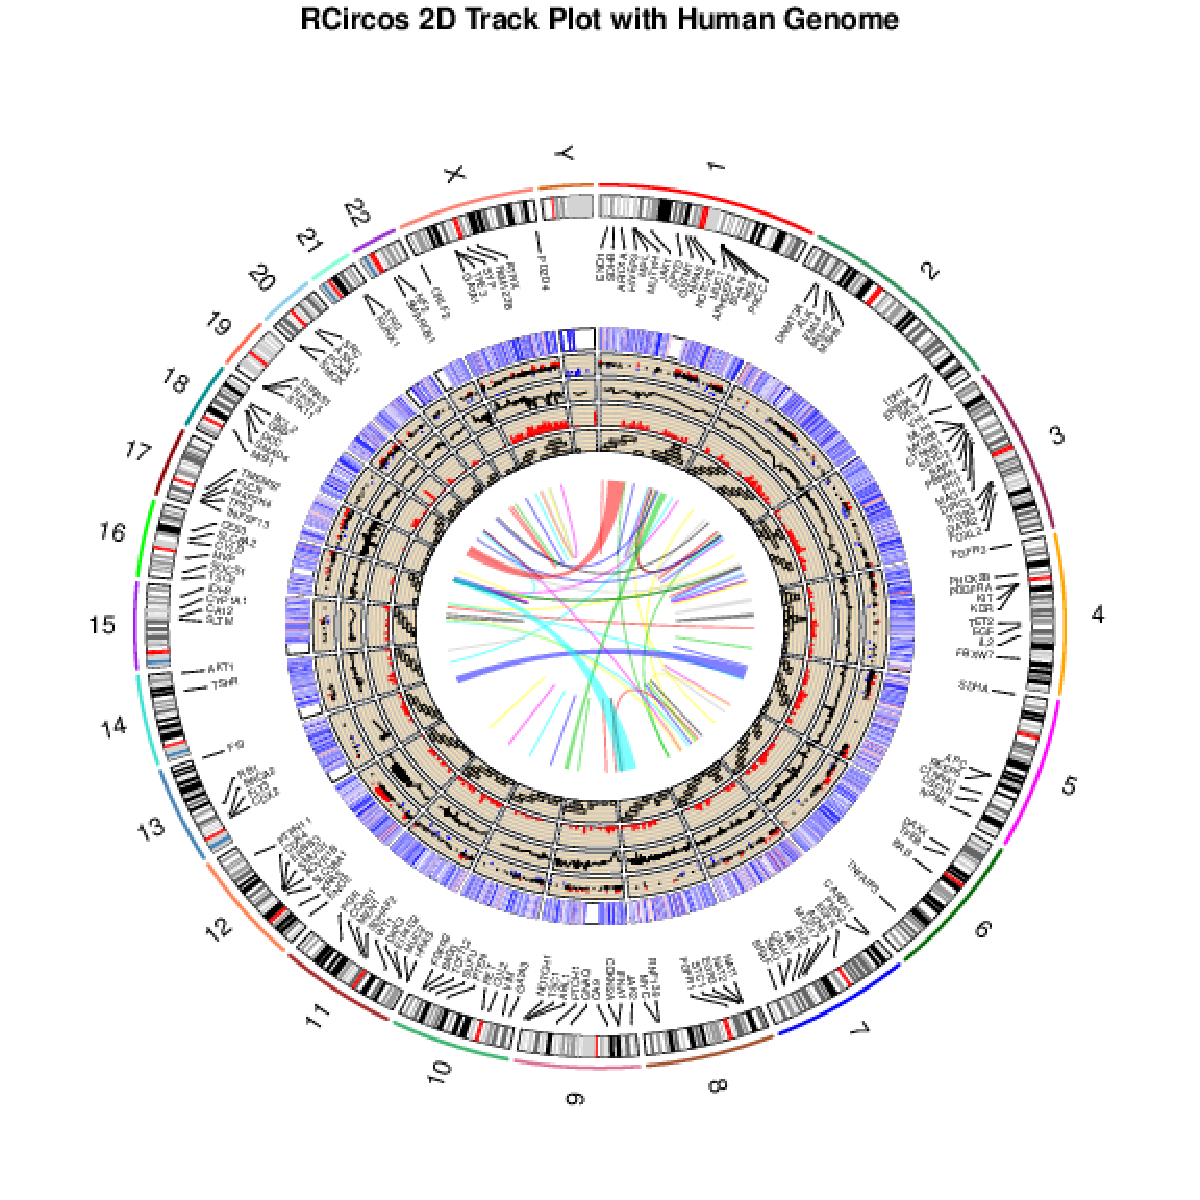
\includegraphics[width=0.9\textwidth]{figure/circos_small.pdf}
        \caption[A human genome diagrammed using the Circos]{A human genome diagrammed using the Circos form. The many tracks of this diagram support a range of graphic forms including scatterplots, heatmaps and histograms all anchored to the ideogram of the 23 chromosomes of the human genome. }
  \label{fig:circos}
\end{figure}

\index{graphic!Circo diagram}

The I/O conference audience, largely comprising software developers,
could hardly be expected to have a detailed interest in cancer genomics.
Their interest was steered toward the immediate availability of
computing power: from 10,000 to 600,000 cores in a few seconds.
\index{machine learning!infrastructures of} Such drastic infrastructural
re-scaling attests to the provocation of the genomic referential. The
Google Compute demonstration is, I would suggest, typical of how
genomes, genes, proteins and biological sciences more generally,
authorize differentiation of individuals, events and things through
machine learning. This differentiation is only hinted at in the Google
I/O keynote address in Hölzle's talk of genomic features, gene
expression and patient attributes.

The only concrete indication of how what was happening in the
demonstration related to machine learning was one mention of the
\texttt{RF-ACE} (Random Forest- Artificial Contrasts with Ensembles)
algorithm. Google's press release emphasises the distribution of
learning across an infrastructure:

\begin{quote}
The primary computation that Google Compute Engine cluster performs is
the \texttt{RF-ACE} code, a sophisticated machine learning algorithm
which learns associations between genomic features, using an input
matrix provided by ISB (Institute for Systems Biology). When running on
the 10,000 cores on Google Compute Engine, a single set of association
can be computed in seconds rather than ten minutes, the time it takes
when running on ISB's own cluster of nearly 1000 cores. The entire
computation can be completed in an hour, as opposed to 15 hours
\autocite{GoogleInc.2012}.
\end{quote}

Google re-purposes an algorithm developed by engineers at Intel
Corporation and Amazon, \index{Amazon} and draws on genomic datasets
provided by the Institute of Systems Biology, Seattle, a doyen of
big-data genomics. The demonstration animates the \texttt{RF-ACE} (a
further development of Breiman's random forests discussed in chapter
\ref{ch:pattern}) by re-drawing a diagram of the genome, and re-draws it
increasingly rapidly as the demonstration scales up to 10,000 cores (or
CPUs). \index{machine learner!RF-ACE} A diagram that normally appears
statically on-screen or on the printed page of a scientific publication
is now animated by an algorithmic process. This confluence of commerce
(Amazon), industry (Intel), media (Google) and genomic science (ISB)
exemplifies the re-inscriptive or transcriptive materiality of machine
learning. \index{Intel!development of RF-ACE}

\section{Genomic knowledges and their
datasets}\label{genomic-knowledges-and-their-datasets}

In the infrastructural materiality of these demonstrations and examples,
whether they come from \emph{Elements of Statistical Learning} or from
Google Compute Engine, the object of knowledge -- genomes, genes,
proteins -- does not figure in terms of its original discipline or
scientific field (typically cancer biology). The scaled-up demonstration
of \texttt{RF-ACE} on Google Compute assembles only a general system of
references between cancer patients, vectorised infrastructures and
predictive classifications. Similarly, the treatment of DNA microarray
data in the slightly earlier examples found in \emph{Elements of
Statistical Learning} does not principally concern cancer biology as
such, but much more the way a group of elements are assembled so as to
permit the production of propositions that cross the threshold of
scientificity. They may just as well cross different thresholds of
knowledge in governmental, market-focused, organisational or managerial
operations.\footnote{In their account of the surprisingly slow shift of
  microarrays towards clinical practice, Paul Keating and Alberto
  Cambrosio identify statistics as a kind of bottleneck:

  \begin{quote}
  The handling and processing of the massive data generated by
  microarrays has made bioinformatics a must, but has not exempted the
  domain from becoming answerable to statistical requirements. The
  centrality of statistical analysis emerged diachronically, as the
  field moved into the clinical domain, and is re-specified
  synchronically depending on the kind of experiments one carries out
  \autocite[49]{Keating_2012}.
  \end{quote}

  What Keating and Cambrosio describe as `becoming answer to statistical
  requirements' I would suggest also entails a transformation of
  statistical requirements in a new operational diagram that reduces
  some of the frictions associated with existing statistical practice.
  This operational diagram is machine learning.
  \index{statistics!biomedical!changes in}
  \index{Keating, Paul!on microarrays}
  \index{Cambrosio, Albert!on microarrays}\index{science!genomics!bioinformatics}}

The plurality of applications can sometimes make it seem that machine
learning arrives at the borders of different domains, and then proceeds
to colonise local knowledges practices. The rule of materiality here
would seem to be an epistemic \emph{terra nullius} appropriation, in
which existing knowledge forms are rapidly extinguished by machine
learners. We have seen previously that ancestral communities of
probabilisation orient the generalization of machine learning (see
chapter \ref{ch:probability}). \index{probabilisation!ancestral}
Research literature published on machine learning since the early 1990s
clusters around problems of plethoric excess -- image recognition,
document classification, market behaviour (as in, working out what
advertisement to show, or whether someone is likely to a buy a
particular product, etc.). These problems position machine learning
amidst regimes of communication, the production of economic value, and
the regularities of statements (or put in more Foucaultean terms, amidst
life, labour and language; see \autocite{Foucault_1992}). Where, amidst
these major regularities, does genomics (arguably the successor of
molecular biology) fit? Almost all of the major machine learners, albeit
supervised or unsupervised, discriminative or generative, parametric or
non-parametric, substantial research activity during the last two or so
decades cross-validate their statements with genomics.
\index{referential!cross-validation of}

\section{\texorpdfstring{The advent of `wide, dirty and mixed'
data}{The advent of wide, dirty and mixed data}}\label{the-advent-of-wide-dirty-and-mixed-data}

We can see this referential cross-validation at work in the shape of
genomic data. The DNA microarray data extensively modelled in the final
chapter of \emph{Elements of Statistical Learning} highlights some
elementary problems of shape associated with genomic data. The
\texttt{iris} dataset \autocite{Fisher_1936}, perhaps the most heavily
used pedagogical dataset in the literature, does not provoke the
infrastructural contortions associated with Google Compute, or for that
matter, the highly sophisticated and quite subtle treatment of gene
expression we find in genomics-related machine learning.

\begin{table}[ht]
\centering
\begingroup\tiny
\begin{tabular}{rrrrl}
  \hline
Sepal.Length & Sepal.Width & Petal.Length & Petal.Width & Species \\ 
  \hline
5.10 & 3.50 & 1.40 & 0.20 & setosa \\ 
  4.90 & 3.00 & 1.40 & 0.20 & setosa \\ 
  4.70 & 3.20 & 1.30 & 0.20 & setosa \\ 
  4.60 & 3.10 & 1.50 & 0.20 & setosa \\ 
  5.00 & 3.60 & 1.40 & 0.20 & setosa \\ 
   \hline
\end{tabular}
\endgroup
\caption{First 5 rows of Fisher's `iris` dataset} 
\label{tab:iris_sample}
\end{table}

It is usual, in working with \texttt{iris,} to construct machine
learners that use the variables from the first four columns shown in
table \ref{tab:iris_sample} to infer the value of the \texttt{Species}
response variable (as seen in Chapter 5, where a decision tree was
constructed using this same dataset). The measurements of petals and
sepals of the irises of the Gaspé Peninsula in Novia Scotia, and their
classification into different species is perhaps a typical mid-twentieth
century biological procedure. Even in the excerpt shown in Table
\ref{tab:iris_sample}, we can see that it is quite narrow as it has only
a few columns, the data is nearly all of one type (measurements of
lengths and widths), and the data is clean (there are no missing
values). \texttt{Iris} is typical of classic statistics and much
biological data prior to genomics in its relatively homogeneity and
distinct partitioning. \index{dataset!\texttt{iris}}

If \texttt{iris} is the conventional statistical form, how does a
genomic dataset differ? One clue comes from descriptions of the
\texttt{RF-ACE} algorithm, first published in 2009. RF\_ACE is attempts
to deal with `modern data sets' that are `wide, dirty, mixed with both
numerical and categorical predictors, and may contain interactive
effects that require complex models' \autocite[1341]{Tuv_2009}. Such
algorithms and the `wide, dirty, mixed' datasets they work on have an
irregular texture, which, I would suggest, we should try to grasp if we
want to understand how genomic data constitutes a complex volume `in
which heterogeneous regions are superposed'
\autocite[128]{Foucault_1972}. Clues to the irregularity of genomic data
come from the various treatments of DNA microarray data in
\emph{Elements of Statistical Learning}. \index{data!wide, dirty, mixed}

Hastie and co-authors introduce one microarray dataset they use in this
way:

\begin{quote}
The data in our next example form a matrix of 2308 genes (columns) and
63 samples (rows), from a set of microarray experiments. Each expression
value is a log-ratio log(R/G). R is the amount of gene-specific RNA in
the target sample that hybridizes to a particular (gene-specific) spot
on the microarray, and G is the corresponding amount of RNA from a
reference sample. The samples arose from small, round blue-cell tumors
(SRBCT) found in children, and are classified into four major types: BL
(Burkitt lymphoma), EWS (Ewing's sarcoma), NB (neuroblastoma), and RMS
(rhabdomyosarcoma). There is an additional test data set of 20
observations. We will not go into the scientific background here
\autocite[651]{Hastie_2009}
\end{quote}

Note that while the number of samples (\textasciitilde{}80) in the small
round blue-cell tumors (\texttt{SRBT}) \autocite{Khan_2001} dataset is
less than the number of flowers measured in \texttt{iris,} the number of
variables presented by the columns in the table (2308) is much greater.
\index{dataset!SRBCT} Hastie and co-authors, like the Google I/O
demonstration, do not `go into the scientific background.' Scientific
knowledge \emph{per se} is not the central concern in machine learning.
Rather, genomic data as a field or emergence and differentiation in the
production of statements
matters.\index{science!knowledge!referentiality of} The original
publication of this dataset in 2001 \autocite{Khan_2001} also made use
of machine learning techniques (neural networks, a major topic in the
next chapter \ref{ch:subjects}), precisely in order to address the
diagnostic problem of distinguishing different tumors types without
resort to new experiments or biological knowledge.\footnote{Khan and
  co-authors write:

  \begin{quote}
  Gene-expression profiling using cDNA microarrays permits a
  simultaneous analysis of multiple markers, and has been used to
  categorize cancers into subgroups 5--8 . However, despite the many
  statistical techniques to analyze gene-expression data, none so far
  has been rigorously tested for their ability to accurately distinguish
  cancers belonging to several diagnostic categories
  \autocite[673]{Khan_2001}
  \end{quote}}

\begin{table}[ht]
\centering
\begingroup\tiny
\begin{tabular}{rrrrrrrrrrrrrrr}
  \hline
GENE1 & GENE2 & GENE3 & GENE4 & GENE5 & GENE6 & GENE7 & GENE8 & GENE9 & GENE10 & GENE11 & GENE12 & GENE13 & GENE14 & GENE15 \\ 
  \hline
0.77 & -2.44 & -0.48 & -2.72 & -1.22 & 0.83 & 1.34 & 0.06 & 0.13 & 0.57 & 1.50 & 0.39 & 1.63 & 0.82 & 0.01 \\ 
  -0.08 & -2.42 & 0.41 & -2.83 & -0.63 & 0.05 & 1.43 & -0.12 & 0.46 & 0.16 & 1.15 & 0.38 & 1.56 & 0.01 & 0.16 \\ 
  -0.08 & -1.65 & -0.24 & -2.88 & -0.89 & -0.03 & 1.16 & 0.02 & 0.19 & 0.50 & 1.39 & -0.53 & 1.61 & -0.21 & 0.08 \\ 
  0.97 & -2.38 & 0.63 & -1.74 & -0.85 & 0.95 & 1.09 & 0.82 & -0.28 & 0.99 & 1.01 & 0.08 & 1.05 & 0.97 & -0.17 \\ 
  0.08 & -1.73 & 0.85 & 0.27 & -1.84 & 0.33 & 1.25 & 0.77 & 0.03 & 0.28 & 1.11 & -0.39 & 1.19 & 0.42 & -0.39 \\ 
   \hline
\end{tabular}
\endgroup
\caption{Small round blue-cell tumour data sample (Khan, 2001)} 
\label{srbct}
\end{table}

The sample of the \texttt{SRBCT} data shown in table \ref{tab:srbct}
does not readily accommodate the width of the dataset. Unlike
\texttt{iris}, the thousands of variables simply cannot be displayed on
a page or screen. \emph{Wide} datasets are quite common in machine
learning settings generally, but particularly common in genomics where
in a given study there might only be a relatively small number of
biological samples but a huge amount of sequencer or microarray data for
each sample. Much genomic data shares this generic feature of
width.\footnote{Importantly, as discussed in Chapter \ref{ch:diagram}
  (in terms of the diagonalization running between different elements of
  code, data, mathematical functions and indexical signs) and in Chapter
  \ref{ch:vector} (in terms of the auratic power of datasets), the fact
  that these datasets can be so readily loaded and accessed via
  bioinformatic infrastructures using code written in \texttt{R} or
  \texttt{Python} is also a notable feature of their advent in the
  machine learning literature. Even a social science researcher can
  quickly write programs to retrieve this data. It attests to several
  decades, if not longer, work on databases, web and network
  infrastructures, and analytical software, all, almost without
  exception, driven by the desire for aggregation, integration,
  archiving and annotation of sequence data that first became highly
  visible in the Human Genome Project of the 1990s. The brevity of these
  lines of code that retrieve and load datasets -- half a dozen
  statements in \texttt{R}, no more -- suggests we are dealing with a
  high-sedimented set of practices, not something that has to be
  laboriously articulated, configured or artificed. Code brevity almost
  always signposts highly-trafficked routes in contemporary network
  cultures. \index{code!brevity of} Without describing in any great
  detail the topography of databases, protocols and standards woven by
  and weaving through bioinformatics, the ready invocation of genomic
  datasets suggests that the mixed, dirty, wide datasets fed to
  algorithms such as \texttt{RF-ACE} or analysed in
  \autocite{Hastie_2009} derives from the layered couplings and
  interweaving of scientific publications and scientific databases
  developed by biological science over the last three decades. As the
  code shows, sequence and other genomic data are available to
  scientists not only as users searching for something in particular and
  retrieving specific data, but to scientists as programmers developing
  ways of connecting up, gathering and integrating many different data
  points into to produce the wide ( many-columned), mixed (different
  types of data), and dirty (missing data, data that is `noisy')
  datasets, datasets whose heterogeneous and often awkward topography
  then elicits and invites algorithmic treatment.}

\begin{figure}
  \centering
      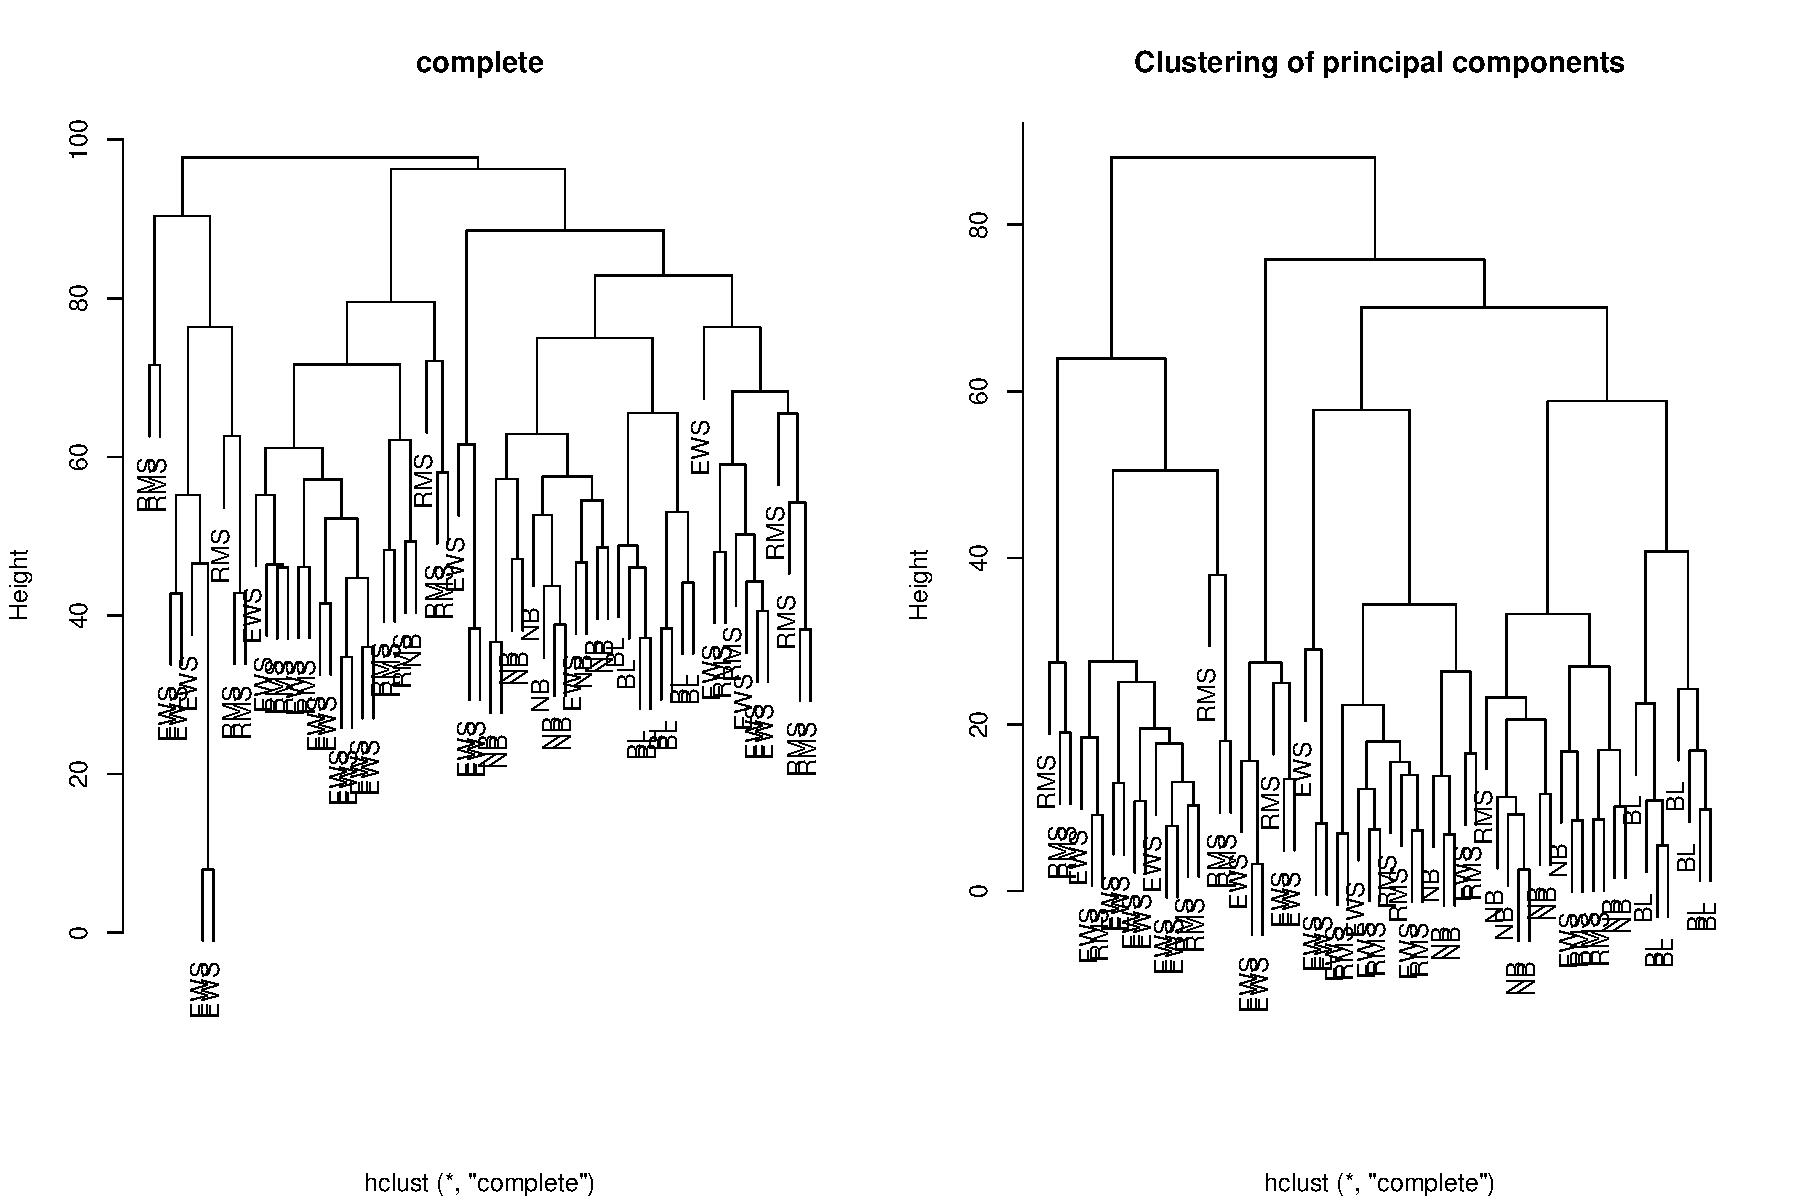
\includegraphics[width=0.9\textwidth]{figure/srbct_cluster-1.pdf}
        \caption{Hierarchical clustering of the SBRCT gene expression data}
  \label{fig:sbrct_clust}
\end{figure}

In contrast to the direct measurements of petals and sepals in the
\texttt{iris} data, the \texttt{SRBCT} data incorporates and diagonally
connects many levels of practice.
\index{datasets!diagrammatic character of} The columns in table
\ref{tab:sbrct} refer to genes whose levels of expression in different
samples are measured and then grouped by comparison to their levels in a
reference sample (see the hierarchical clustering
\index{machine learner!hierarchial clustering} of the data shown in
figure \ref{fig:sbrct_clust}.) Even the identification of the several
thousand genes whose levels of expression are measured by the microarray
experiments presupposes much preceding work on DNA sequences and the
identification of protein-coding DNA regions amidst the highly
repetitive vector of the genome sequence. Highly leveraged
infrastructures for access to biological data underpin such datasets.
Considered more diagrammatically, genomes in many ways becomes less
linear or flat than the bare base DNA sequences might suggest.

\section{Cross-validating machine learning in
genomics}\label{cross-validating-machine-learning-in-genomics}

The linear sequences of DNA data mix and diffuse partly through the
archival accumulation that allows them to be superimposed, annotated and
layered, but also through the many efforts to traverse their expanded
volume using classifiers and predictive models. A recent review in the
journal \emph{Genomics} highlights the increasing bearing of machine
learning techniques on genomic science:

\begin{quote}
High-throughput genomic technologies, including gene expression
microarray, single Nucleotideide polymorphism (SNP) array, microRNA
array, RNA-seq, ChIP-seq, and whole genome sequencing, are powerful
tools that have dramatically changed the landscape of biological
research. At the same time, large-scale genomic data present significant
challenges for statistical and bioinformatic data analysis as the high
dimensionality of genomic features makes the classical regression
framework no longer feasible. As well, the highly correlated structure
of genomic data violates the independent assumption required by standard
statistical models\autocite[323]{Chen_2012}. \index{correlation}
\index{statistics!limits of!genomic data}
\end{quote}

Commentary on the `highly correlated structure,' not just the volume, of
genomic data, points to another referential operation concerning the
differentiation of things. \index{referential!differentiation in} Many
such statements highlight the incompatibility between a surging
multiplicity of data forms and the constraints of existing statistical
modelling techniques (`standard statistical models'). So for instance,
Chen and co-authors recommend the use of the random forest (RF) because
it:

\begin{quote}
is highly data adaptive, applies to ``large p, small n'' problems, and
is able to account for correlation as well as interactions among
features. This makes RF particularly appealing for high-dimensional
genomic data analysis, \ldots{} including prediction and classification,
variable selection, pathway analysis, genetic association and epistasis
detection, and unsupervised learning \autocite[323]{Chen_2012}
\index{machine learner!random forest!use in genomics}
\end{quote}

Familiar machine learning vectorisation keywords such as `large p, small
n' and `high dimensional' pepper their recommendations. But the key
terms on the genomics side of this formulation would perhaps be `pathway
analysis', `genetic association,' and `epistasis.' Such biological terms
point to forms of relationality associated with biologically interesting
processes. Epistasis for instance broadly refers to linked gene action,
a process that has been difficult to study before high-throughput
methods of functional genomics brought shifting patterns of gene
expression to light. \index{science!genomics!epistasis} In contemporary
genomic science, these biological processes are increasingly understood
in terms of eliciting and modelling the relations between
\emph{features} of genomic datasets in order to classify and predict
biological outcomes.

How does machine learning differ from the statistical practice that has
underpinned much of modern biology? The analysis of \texttt{SRBCT} gene
expression in \emph{Elements of Statistical Learning} is symptomatic of
a mutual articulation, a cross-validation that entangles genomics and
machine learning. \index{referential!cross-validation of} The overt
arrival of machine learning techniques in genomic research was initially
largely concerned with the problem of variations in gene expression (
and in fact, nearly all of the analysis of genomic data in
\emph{Elements of Statistical Learning} explicitly deals with various
cases of gene expression). \index{dataset!SRBCT} On the one hand, the
genomics data promises legibility of all the genes in a given organism
(\textasciitilde{}20,000 for humans). On the hand, the pattern of
activity of these genes in time, or any particular point in the life of
an organism, cannot be read from the genome but only in time-varying
expression, the changes in state and the variations in closely similar
genomes. \index{genomics!problem of gene expression}

Compared to the refined algorithmic craft of whole genome assembly
\autocites{Venter_2001}{Myers_2000}{Pevzner_2001}, the handling of the
problem of gene expression in machine learning settings can seem rather
crudely lacking in biological specificity. Hastie and co-authors almost
deprecate scientific knowledge: `we will not go into the scientific
background here.' Like the authors of the original scientific study
\autocite{Khan_2001}, \emph{Elements of Statistical Learning} treats
gene expression profiling largely as a problem of learning to classify
differences in disease or other health-related conditions. The many gene
expression studies seek to discriminate between different conditions,
diseases, or pathologies on the basis of differing levels of gene
expression. For machine learners, each gene is a variable whose levels
of expression in a given sample may help identify what type that sample
belongs to. In the case of the \texttt{SRBCT} data, the types include
lymphomas, sarcomas and neuroblastomas.

Like Chen, \emph{Elements of Statistical Learning} begins by addressing
the problem of the shape of the data. `Since \(p\gg N\)' write Hastie
and co-authors, `we cannot fit a full linear discriminant analysis (LDA)
to the data; some sort of regularization is needed'
\autocite[651]{Hastie_2009}.
\index{machine learner!linear discriminant analysis!not applied to gene expression}
\index{machine learning!regularization in} What is this
\gls{regularization}? Like the re-distribution of classification into a
randomised population of machine learners (see chapter
\ref{ch:probability}, regularization governs an potentially unruly
plurality through a form of training and observation. Michel Foucault
describes the advent of disciplinary power partly in terms of enclosure
or individualizing observation, but also in terms of techniques of
supervising, examining and above all, \emph{regularizing} conduct. He
writes:

\begin{quote}
Shift the object and change the scale. Define new tactics in order to
reach a target that is now more subtle but also more widely spread in
the social body. Find new techniques for adjusting punishment to it and
for adapting its effects. Lay down new principles for regularizing,
refining, universalizing the art of punishing
\autocite[89]{Foucault_1977}
\index{power!disciplinary!regularization in}
\end{quote}

Foucault's description of regularization as a technique of disciplinary
power -- the formation that emerged in the late 18th century as a way of
ordering `massive or transient pluralities' (143) in Western European
societies -- seems a long way from microarray gene expression data.
\index{Foucault, Michel!disciplinary power}
\index{machine learning!regularization in} Yet the data in genomic and
other referentials (transactions, social media, etc.) displays some of
the traits -- massiveness, transience, plurality -- that Foucault
identifies as key targets of regulation for the operations of
disciplinary power focused on the social body or populations.
\index{population!as social body} The `target,' a term often used in
machine learning to describe the type, group or response being modelled,
in genomics is often subtle variations (in gene expression, in
phylogeny, in pathogenesis), and these variations are widely dispersed
in genomic sequence data and in the populations it stems from.
\index{data!variable!target|see{data!variable!response}} Foucault's
account of supervision (\emph{surveiller}) and penalisation as
disciplinary techniques responding to `popular illegality'
\autocite[130]{Foucault_1977} dwells on the capillary network of
observations, examining, ranking, test and gradation that adapt to the
surging multiplicities by ordering them in tables. While the tables of
data (see Table \ref{tab:srbct} in the microarray gene expression
datasets suggest the persistence of the same technique of ordering
multiplicities through partitioned observations, the \emph{cells} no
longer target contain individuals under observation but focus on the
attributes of a multiplicity in movement, the human genome for instance
in its many functional states. \index{referential!regularization in}

`Shift the object and change the scale,' Foucault writes, in describing
how partitions, segmentations, forms of enclosure, and above all, ranked
classifications target a more subtly distributed nexus of relations in
disciplinary power. Often understood in terms of enclosure and
surveillance, disciplinary power, according to Foucault, operates
through ranking: `discipline is an art of rank, a technique for the
transformation of arrangements' \autocite[145]{Foucault_1977}.
\index{classification!as ranking} `Regularize in a way that
automatically drops out features that are not contributing to the class
predictions,' Hastie and co-authors write \autocite[652]{Hastie_2009} in
describing how regularization deals with the problem of too many
variables in the microarray datasets. In the many different techniques
that \emph{Elements of Statistical Learning} brings to bear on the
problem of gene expression -- diagonal linear discriminant analysis,
nearest shrunken centroids, linear classifiers with quadratic
regularization, regularized discriminant analysis, regularized
multinomial logistic regression, support vector classifier --
essentially the same ordering movement occurs. Regularization re-scales
the excessive potential relations of the hyperobject -- the patterns of
expression of genes associated with different types of tumours -- by
shrinking or dropping the weights of parameters of each gene in the
model and examining the effect on the predictions that result. The
coefficients or weights of parameters in the model, the \(\beta_p\)
values, are ranked by importance, and then either reduced (\(L_2\)
regularization) or eliminated (\(L_1\) regularization) if they
contribute little to the predictive accuracy of the machine learner.
Learning here takes the form of regularization.
\index{machine learning!regularization}
\index{hyperobject!regularization of}

A technique called `lasso regression' displays features that might help
us grasp how machine learners regularize genomic data.
\index{machine learner!linear regression!lasso} Remember that the linear
regression model with its diagonal line or plane running through vector
space provides the underlying intuition for many machine learners. We
have seen the function in Equation \ref{eq:linear_model4} several times
already in different variations, including logistic regression used for
classification of types or groupings.

\begin {equation}
\label {eq:linear_model4}
\hat{Y} = \hat{\beta_0}  + \sum^p_{j=1} X_j \hat{\beta_j}
\end{equation}

In gene expression models, the values of \(\beta\) shown in equation
\ref{eq:linear_model4} map on to the different levels of expression of
the many genes indexed by the \(p\) columns of the microarray dataset.
The model tests how different patterns of gene expression associate with
different tumour types. As we have already seen, the number of
combinations of genes associated with different tumour types vastly
outweighs the number of samples.

The regularized version of the linear regression framework known as
`lasso' -- Least Absolute Shrinkage and Selection Operator -- introduces
a different form of training and observation of model construction. This
train hinges on the lasso penalty shown in equation
\ref{eq:lasso}\footnote{The original publication of the lasso technique
  in a paper entitled `Shrinkage and Selection via the Lasso'
  \autocite{Tibshirani_1996} has been heavily cited in subsequent
  literature.
  \href{http://scholar.google.co.uk/scholar?hl=en\&q=tibshirani+1996+lasso}{Google
  Scholar} counts around 13,000 citations. For a paper published in the
  \emph{Journal of the Royal Statistical Society}, this is surprisingly
  high, but attests, I would suggest, to the intense interest in
  renovating linear models for new problems such as image recognition or
  tumour classification. Somewhat surprisingly, given its heavy usage in
  other scientists, Andrew Ng's CS229 machine learning course at
  Stanford University doesn't mention the lasso.}
\index{machine learner!Least Absolute Shrinkage and Selection Operator}

\begin {equation}
\label {eq:lasso}
\widehat{\beta}^{lasso} = argmin_\beta\left\{ \frac{1}{2}\sum_{i}^{N}{(y_i - \beta_0 - \sum_{j=1}^{p}{x_{ij}\beta_j})^2}+ \lambda \sum_{j=1}^{p} \vert \beta_j \vert \right\}.
\end{equation}

\begin{quote}
\begin{quote}
\autocite[68]{Hastie_2009}
\end{quote}
\end{quote}

Equation \ref{eq:lasso} is notable for the way that it subjects the
familiar `residual sum of squares' way of calculating the coefficients
to the `penalty' carried by the last part of the equation
\(\sum\limits_i^p\vert\beta_j\vert\).
\index{machine learner!Ordinary Least Sum of Squares} As Hastie and
co-authors write, `the lasso does a kind of continuous subset
{[}feature{]} selection' \autocite[69]{Hastie_2009}. As always
\(argmin_\beta\) suggests that the algorithm should optimise the set of
values for \(\beta\) that minimize the overall value of the function. It
balances the costs of reducing the sum of residual errors shown in the
first half of the equation, and minimizing the sum of the absolute
values of the model parameters \(\beta_j\) in the second part of the
function. The optimizing double movement re-shapes its expression of the
data along a diagonal line drawn as the algorithm gradually introduces
and scales all of the features in the vector space \(\mathbf{X}\), only
allowing those variables or features to remain in the set that help
minimize the difference between the predicted response and the actual
response. \index{diagrammatic!diagonal} (Figure \ref{fig:lasso} makes
something of this scaling diagrammatically visible. In this diagram, the
various diagonal lines show how values of coefficients grow and
sometimes diminish as the \texttt{lasso} process runs. Vertical lines
show steps as new variables are included in the model with different
values of the control parameter \(\lambda\). )

\begin{figure}
  \centering
      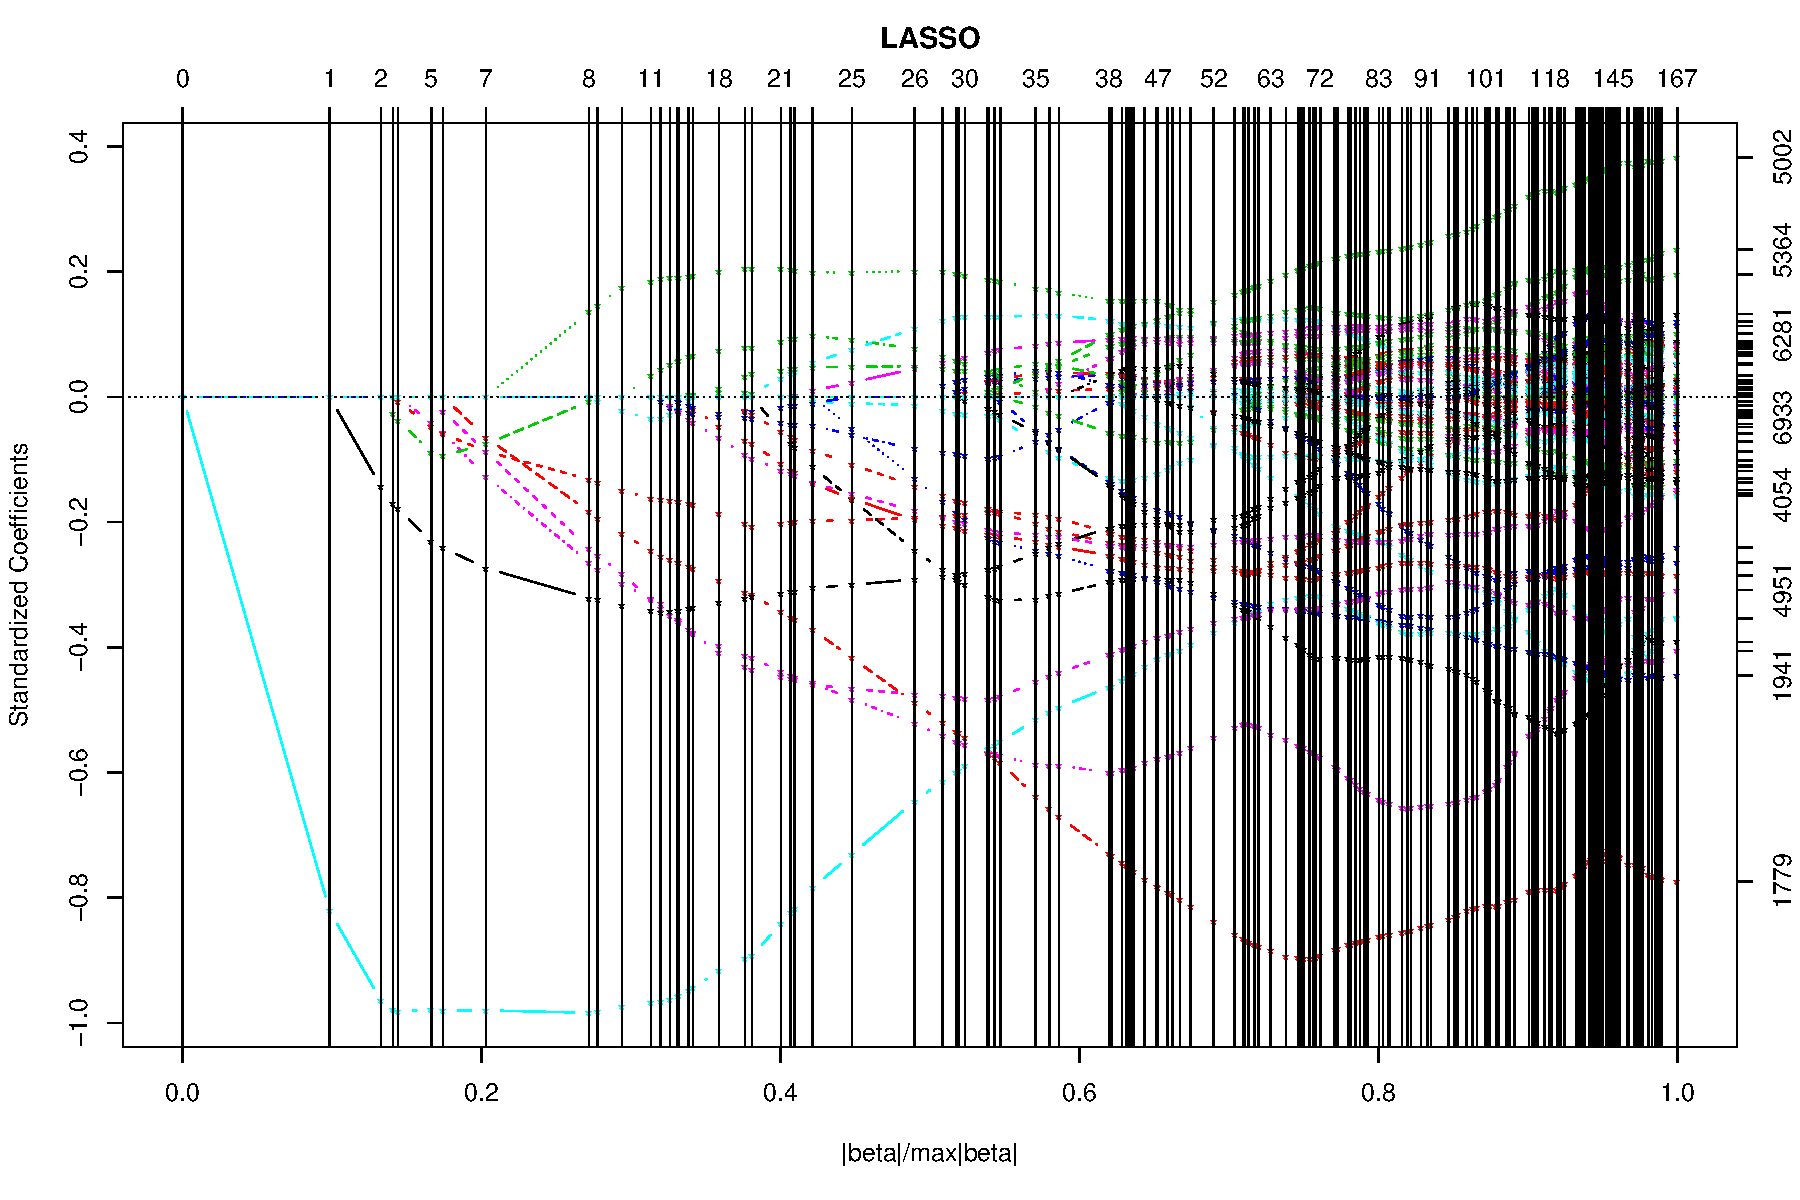
\includegraphics[width=1.0\textwidth]{figure/lasso-1.pdf}
        \caption[Shrinkage paths]{Shrinkage path of coefficients for Lasso regression on (Golub,1999) leukemia data}
  \label{fig:lasso}
\end{figure}

Regularization sometimes radically changes the object. In Figure
\ref{fig:lasso}, these changes become a matter of diagrammatic
observation. Comparing eight different methods for analyzing the
microarray cancer data from \autocite{Ramaswamy_2001}, Hastie reports
that `lasso regression (one versus all)' selects 1,429 of the 16,063
genes in the dataset. The shifted-rescaled object, a set of 1400 genes,
or in the case of the `elastic-net penalized multinomial' model that
uses only 384 genes, highlights a drastically reduced subset of the
original object. A regularized genome of 384 genes suggest a much more
targeted set of interventions than 16,000.

\section{Proliferation of
discoveries}\label{proliferation-of-discoveries}

Despite all the infrastructural cross-validation and regularization of
plural expression, machine learning does not stabilise genomes as data
objects. In many ways, it gives rise to further transformations and
variations, and new sources of error.\footnote{One important difficulty
  is the increasingly visible presence of variations in genomes. These
  variations first become visible after the assembly of whole genome
  sequences. Genomes of individuals of the same species vary in having
  slightly different versions of the genes (alleles), many of which
  differ only by single nucleotide base pairs. Whole genome sequencing
  made these differences, known as single nucleotide polymorphisms
  (SNPs), much more apparent. They occur in their tens of millions in
  the human genome (some 100 million are reported in the NCBI dbSNP
  database). In coding regions, SNPs may occasion changes in protein
  structure; in non-coding regions that can affect how gene expression
  occurs or is regulated. Like genes, SNPs can be detected using
  microarrays. SNP microarrays are commonly used in genome-wide
  association studies (GWAS) that explore complex genetic traits and
  conditions. SNP-based DNA microarrays measure the occurrence of
  millions of SNPs in a given biological sample.
  \index{genomes!single nucleotide polymorphism}} If on the one hand,
machine learners offer to regularize transient multiplicities (such as
gene expression in complex disorders), on the other hand, within
genomics itself, machine learning exhibits considerable epistemic
instability that itself needs to be regulated.
\index{machine learning!regularization of}

For instance, the US Food and Drug Administration has since 2003
conducted a study of data analysis techniques for microarray data:

\begin{quote}
The US Food and Drug Administration MicroArray Quality Control (MAQC)
project is a community-wide effort to analyze the technical performance
and practical use of emerging biomarker technologies (such as DNA
microarrays, genome-wide association studies and next generation
sequencing) for clinical application and risk/safety assessment
\autocite[292]{Parry_2010}. \index{science!genomics!MAQC study}
\end{quote}

Phase I of the US Federal Drug Administration-led MAQC addressed many
issues of data analysis in the context of the clinical applications of
gene expression analysis using microarrays. The primary statistical
issue there was minimizing the `false discovery rate'
\autocite[S1]{Slikker_2010}, a typical biostatistical problem.
\index{error!false discovery rate} In its second phase known as MAQC-II
starting in 2007, however, the focus rested on the construction of
predictive models for `toxicological and clinical endpoints \ldots{} and
the impact of different methods for analyzing GWAS data'
\autocite[2]{Slikker_2010}. On both the clinical and GWAS fronts, the 36
participating research teams tried out many predictive classifier
models. \index{data!variations} \index{dataset!MAQC-II}

\index{machine learner!\textit{k}-nearest neighbours} In the shift from
MAQC-I to MAQC-II, the problem of variations in the predictions produced
by the machine learning models moved to center-stage. The problem of
variation arises not because any of the different modelling strategies
used in machine learning gene expression datasets are wrong or
erroneous, but because every model transforms the `feature space'
\autocite[292]{Parry_2010} in a different way (as we saw in chapter
\ref{ch:pattern} in discussions of different treatments of
dimensionality). In the MAQC-II consortium, teams were tasked to build
`classifiers' to predict whether a given sample or case belongs to a
`normal' or `disease' group. The most popular classifier in the MAQC
consortium was the \emph{k} nearest neighbours model: `{[}a{]}mong the
19,779 classification models submitted by 36 teams, 9742 were k-nearest
neighbor-based (KNN-based) models (that is, 49.3\% of the total)
\autocite[293]{Parry_2010}. But, these models varied greatly in their
predictions: 'there have been large variations in prediction performance
among KNN models submitted by different teams' (293). Not only the
genome itself varies, but the population of machine learners show
variations.\index{population!machine learners!variation of|(}
\index{machine learning!error!bias-variance}

What accounts for this variation? First of all, the teams did not build
single models. As is the norm in machine learning, they iterated over
thousands. In their attempt to normalise the variations of their models,
one of the research groups in MAQC-II write that `for clinical end
points and controls from breast cancer, neuroblastoma and multiple
myeloma, we systematically generated 463,320 \emph{k-nn}
{[}\emph{k}-nearest neighbour{]} models by varying feature ranking
method, number of features, distance metric, number of neighbors, vote
weighting and decision threshold' \autocite[292]{Parry_2010}. A striking
proliferation of models on a population-scale strives to tame the
variations of predictive models. The number of predictive models
constructed here rivals the number of SNPs typically assayed by the
microarrays. It seems as if not only the dimensions of the data have
vastly increased, but the population of models. This population exhibits
many of the problems of variation, irregularity, transience and
plurality found in the genomic referential itself.
\index{population!machine learners!variation of|)}

\section{Variations in the object or in the machine
learner?}\label{variations-in-the-object-or-in-the-machine-learner}

\begin{figure}
  \centering
      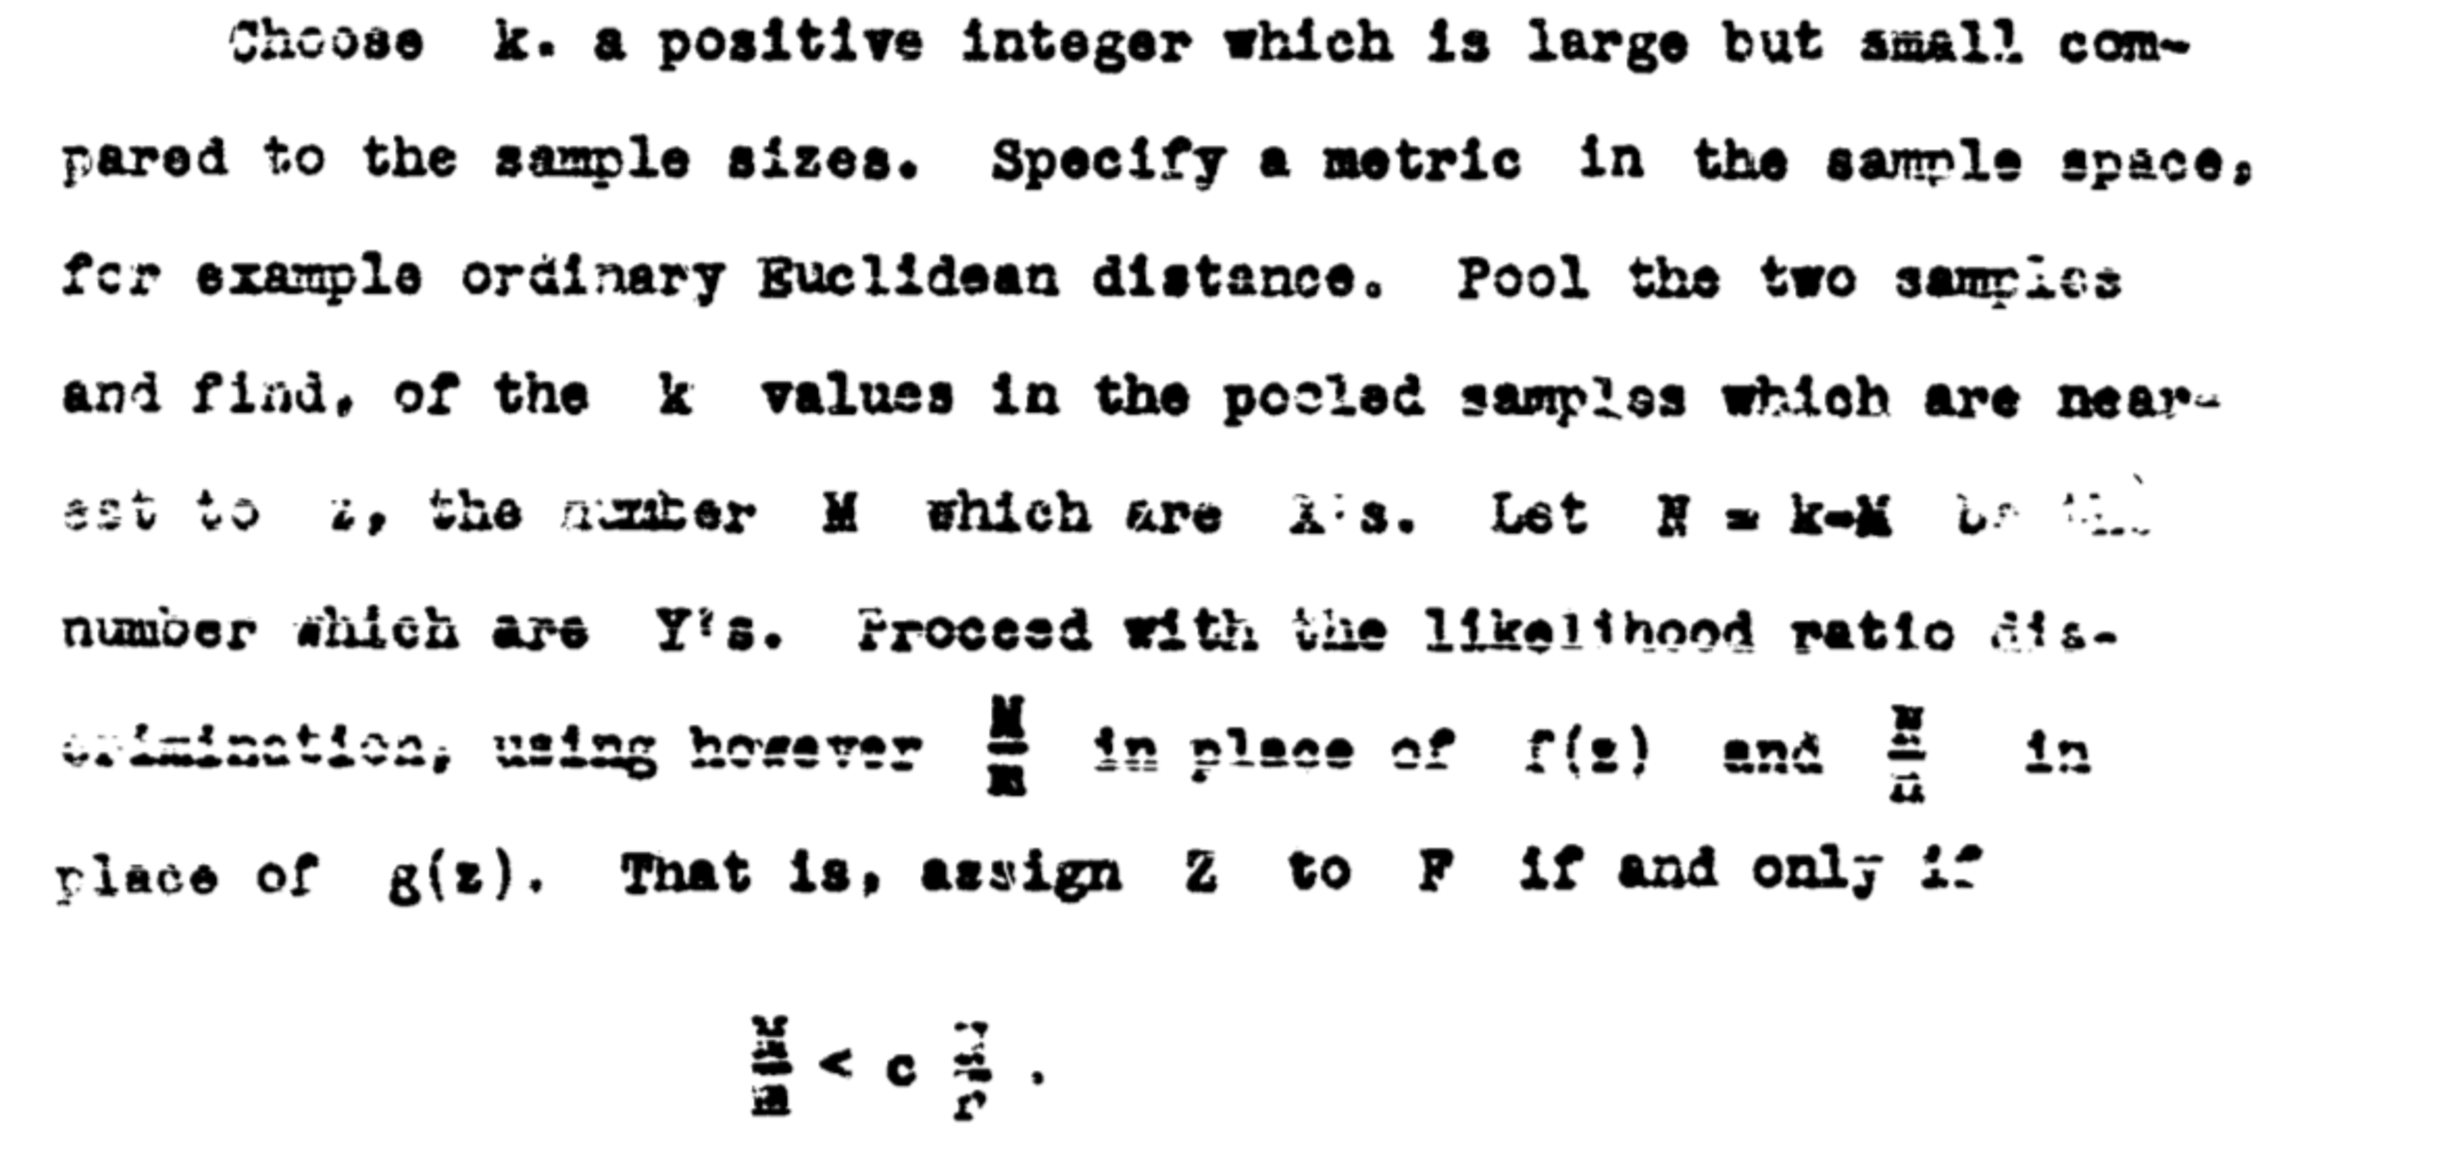
\includegraphics[width=0.99\textwidth]{figure/fix_hodges_excerpt.pdf}
        \caption[Formulation of k-nn model]{The earliest formulation of the \textit{k}-nearest neighbours model from Evelyn Fix and Joseph Hodges' work \cite{Fix_1951}}
  \label{fig:fix_excerpt}
\end{figure}

`The method of k-nearest neighbors makes very mild structural
assumptions: its predictions are often accurate but can be unstable'
write Hastie and co-authors \autocite[23]{Hastie_2009}. The algorithm,
first described by Evelyn Fix\index{Fix, Evelyn} and Joseph Hodges
working at Berkeley in the early 1950s \autocite{Fix_1951}, is extremely
simple in mathematical terms.\footnote{Fix and Hodges frame their
  suggestion of the \emph{k} nearest neighbour model in this way: `there
  seems to be a need for discriminative procedures whose validity does
  not require the amount of knowledge implied by by the normality
  assumption, the homoscedastic assumption, or any assumption of
  parametric form. The present paper is, as far as the authors are
  aware, the first one to attack subproblem (iii): can reasonable
  discrimination procedures be found which will work even if no
  parametric form can be assumed?' \autocite[7]{Fix_1951}. Subproblem
  (iii) in this quote refers to the challenge of deciding which of two
  populations an observed case belongs to if we know nothing about the
  parameters describing the two populations.
  \index{machine learner!\textit{k}-nearest neighbours!history}}
Equation \ref{eq:knn} shows almost the entire algorithm:
\index{machine learner!\textit{k}-nearest neighbours}

\begin {equation}
\label {eq:knn}
\hat{Y}(x) = \frac{1}{k}\sum_{x_i \in N_k(x)}y_i
\end {equation}

`where \(N_k(x)\) is the neighbourhood of \(x\) defined by the \(k\)
closest points \(x_i\) in the training
sample'\autocite[14]{Hastie_2009}. The algorithm effectively takes the
average values of points in the neighbourhood \(N_k\), and uses that
value to predict the result (a classification or a prediction) for a
given point or instance. As Hastie and co-authors put it, the
neighbourhood is just those \(k\) points near the case under
consideration. The assumption here, as in nearly all machine learners
transforming the vector space, is that proximity in vector space implies
similarity in class or grouping. \index{differences!proximity} This
assumption was formally described in the late 1960s in another highly
cited paper \autocite{Cover_1967} on `Nearest Neighbour Pattern
Classification.' Neighbouring points in the vector-space are more
similar than those at a distance. As equation \ref{eq:knn} shows,
\emph{k} nearest neighbours seems to have only one parameter, the value
\(k\), the number of neighbours that a given model includes in its
definition of a `neighbourhood.' In contrast to the linear forms of the
models (formulated in equations \ref{eq:lasso} or
\ref{eq:linear_model4}), equation \ref{eq:knn} seems to require little
training, supervision or regularization to work as a classifier. While
nearly all of the models discussed in this and earlier chapters work
with a smooth functional form of the line or curve as their basic way of
transforming vector space, \emph{k} nearest neighbours generates highly
non-linear boundaries wending their way through the data. Because they
are not guided by parameters (apart from the value of the
hyper-parameter \(k\)\index{parameters!hyper-parameter}), these
boundaries can be unstable.

\begin{figure}
  \centering
      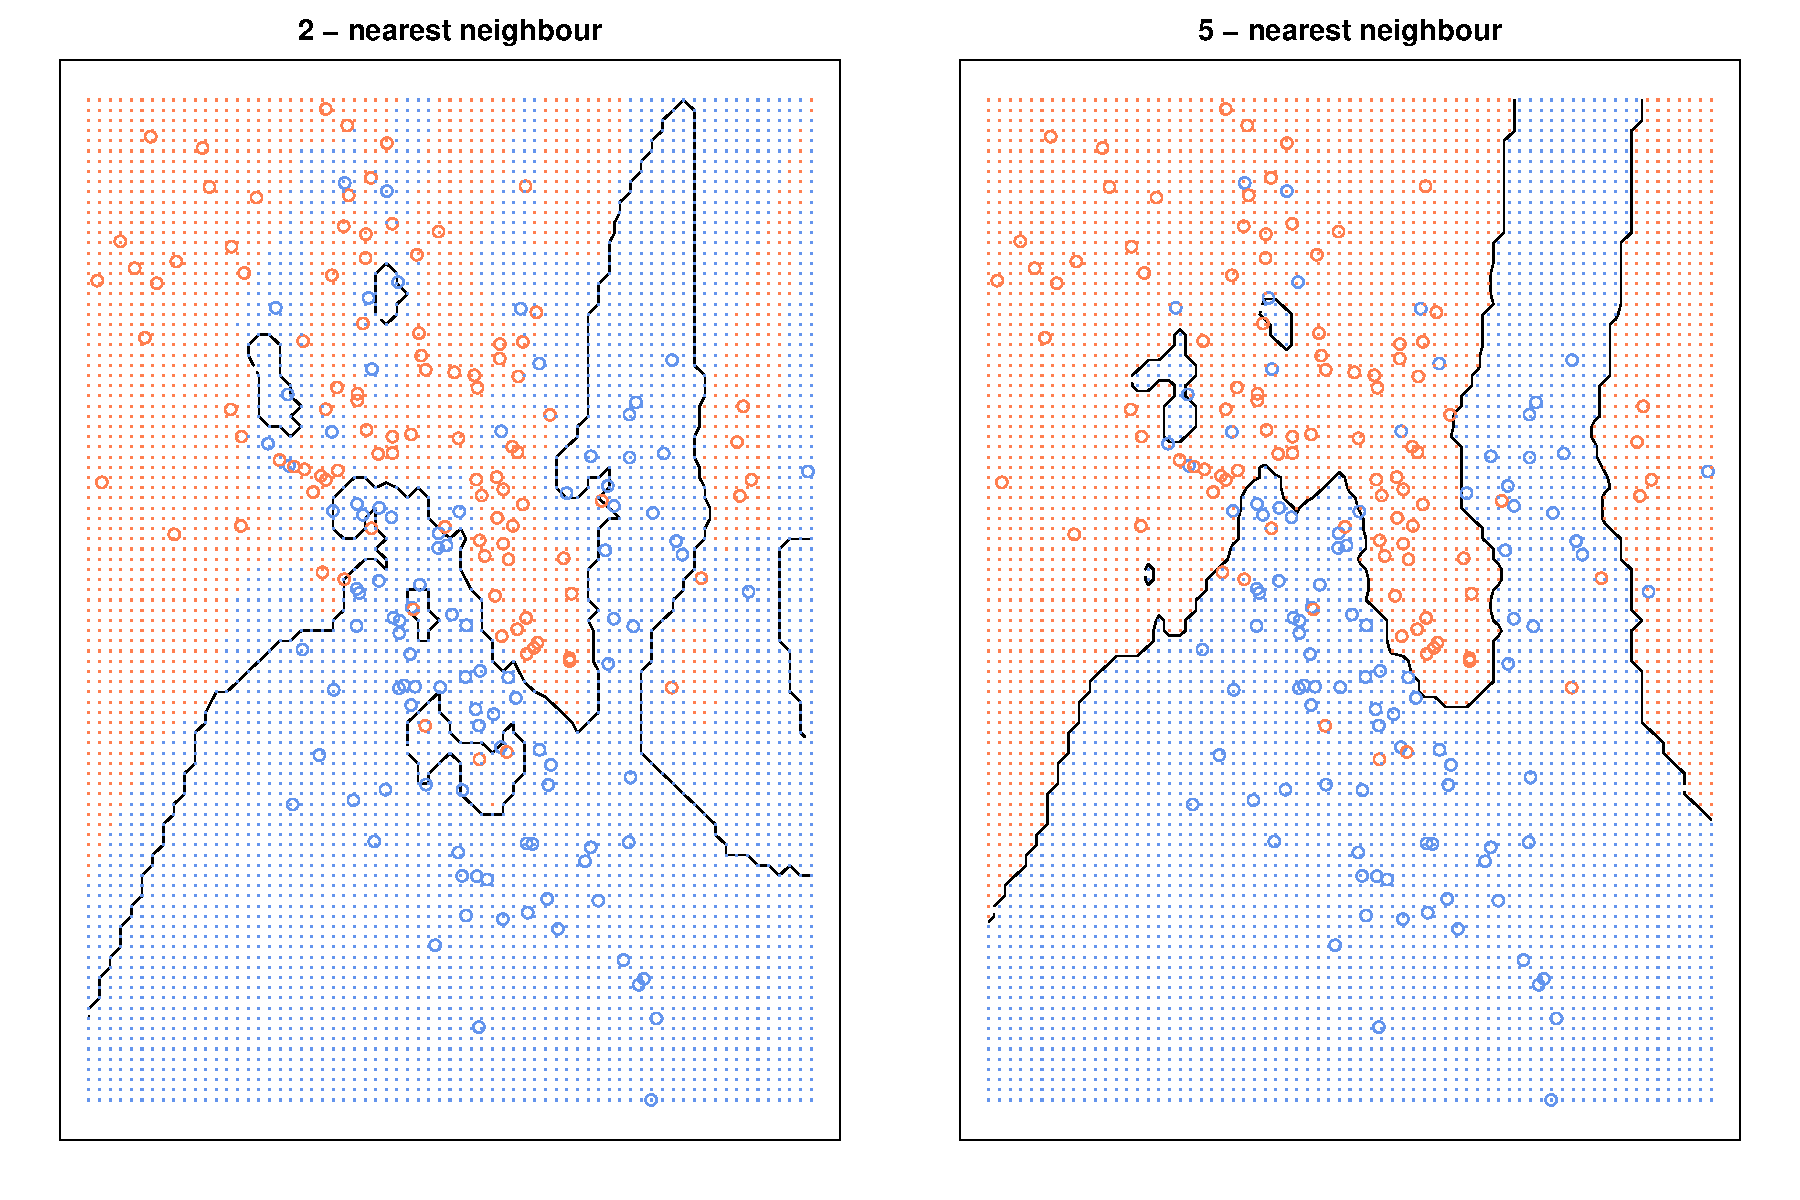
\includegraphics[width=0.9\textwidth]{figure/knn-1.pdf}
        \caption[KNN models for simulated data in two classes]{KNN models for simulated data in two classes. The decision boundary that separates the two classes is non-linear for both versions of the KNN model. For $k=5$, the decision boundary is more non-linear than for $k=b$ }
  \label{fig:knn}
\end{figure}

\index{machine learner!k-nearest neighbours}

Even when data belongs to two classes (e.g. \texttt{normal} vs.
\texttt{not-normal}), decision boundaries produced by \emph{k}-nn can be
unstable. The example in figure \ref{fig:knn} shows two models, one for
\(k=5\) and the other for \(k=2\). Each model examines the relations
between 2, 5 points in deciding whether a particular case belongs to one
class or another. While \emph{k-nn} constructs local clusters and traces
out an irregular decision boundary, this classificatory power comes at
the cost of instability. (This is another version of the bias-variance
decomposition of machine learner errors discussed in chapter
\ref{ch:probability}.)

More data, or wider data exacerbates the instability. As dimensions or
features in the dataset increase, the local neighbourhood needed to
capture a fraction of the volume of the data expands. It becomes more
likely that most sample points will lie close to the boundary of the
sample space, where they will be affected by the neighbouring space. The
result is that `in high dimensions all feasible training samples
sparsely populate the input space' \autocite[23]{Hastie_2009}. Because
\emph{k-nn} allows for non-linear interactions between features, for
instance, small differences in the number of points in particular
neighbourhoods can drastically affect some stretches of the boundaries
(as we see in comparing the right and left hand plots in figure
\ref{fig:knn}). These kinds of topological instability account for the
propensity of machine learning treatments of feature-rich genomic data
to produce accurate but unstable predictions. We can begin to see how a
MAQC-II team might have produced 463,000 \emph{k} nearest neighbour
models in an effort to normalise and regulate predictive predictions.
The price of accurate predictivity in genomics is variation in
prediction.

\section{Whole genome functions}\label{whole-genome-functions}

Cores, microarrays, SNPS,and many models; infrastructural scaling,
biological variation and the populations of unruly machine learners
entwine in referential entanglement. If genomes are scientific
hyperobjects (with epistemic, speculative, financial and biopolitical
resonances), what part does their referential cros-validation with
machine learning play in the transformation of
knowledge?\index{knowledge!referentials in}

Genomic data -- beginning with DNA sequences, then levels of gene
expression, followed by genome wide association studies of small
mutations -- has been a constant \(p \gg N\) antigen in machine
learning. Techniques of regularization -- the lasso -- of linear models
discussed in this chapter came to light, and were first demonstrated on
genomic data produced in the mid-1990s. Throughout the ongoing
development and enrichment of DNA and protein sequencing techniques,
replete with a vast and quite dynamic bioinformatic infrastructure,
machine learning and genomics have been cross-validating in practice.
Scientists, statisticians, datasets and machine learners traffic between
genomics and machine learning at almost every level, ranging from the
sequence assembly to testing and analysis of DNA data in clinical
settings. In genomics, elementary practices of aligning and assembling
sequences into whole genomes were re-configured probabilistically
through machine learning models.

Almost every subsequent development in genomics (and related fields such
as proteomics) follows a referential flow of materializing
transcription, infrastructural cross-validation, and regularizing
differentiation. \index{referential!processes of the} An entity whose
constitution is thoroughly dependent on prediction or algorithmic
classification displays variations and grouping (such as gene
expression, the linkage disequilibrium of SNPs, the seeming abundance of
junk DNA that is actually functional, etc.) that attract further efforts
to differentiate, regularize, and classify ever more subtly distributed
differences. Elementary practices in contemporary genomics such as
sequence alignment were explicitly formulated as generative models to be
constructed using algorithms such as expectation maximization. As we see
in the vignettes from \emph{Elements of Statistical Learning}, the
demonstration of Google Compute cloud computing, or for that matter in
the myriad publications in both machine learning and life science
journals that make use of support vector machines, neural networks,
linear discriminant analysis or random forests, machine learning
establishes a new set of conditions for the exercise of scientific
research, and configures new kinds of statements, new types of objects
(genomes in particular are difficult to conceive without their
probabilistic modelling) and, as will be discussed in the next chapter,
subject positions (bioinformaticians, computational biologists, data
scientists and others). \index{machine learning!positivity of}

What is at stake in approaching machine learning in a scientific setting
like genomics? Foucault writes that `we should distinguish carefully
between \emph{scientific domains} and \emph{archaeological territories}'
\autocite[183]{Foucault_1972}.
\index{knowledge!science!relation between} Knowledge stems from the
practices that connects objects, field, subjects, statements, and
institutions. Sciences are always localized within a field of knowledge
that may exceed, and mutate in ways that alter, local sciences. Science,
for Foucault and perhaps for science studies more generally, needs
knowledge practices that exceed, surround and indeed do something
different to science. Machine learning is just such an operational
formation.

Could we pose or address any normative questions by becoming aware of
and articulating machine learning with science with greater clarity?
Genomic science, in its cross-validation with machine learning, displays
some of the tendencies to reduce divergences and to corral differences
typical of knowledge economies more generally. The philosopher of
science, Isabelle Stengers writes:

\begin{quote}
with the knowledge economy, we may have scientists at work everywhere,
producing facts with the speed that new sophisticated instruments make
possible, but that the way those facts are interpreted will now mostly
follow the landscape of settled interests. \ldots{} We will more and
more deal with instrumental knowledge. (Stengers 2011:377)
\index{Stengers, Isabelle!science!knowledge economy}
\index{knowledge!economy}
\end{quote}

As we see in the 600,000 cores of Google Compute applied to exploration
of associations in cancer genomics using random forests, or the lasso
applied to microarray SNP data, machine learning rapidly produces facts.
Stengers suggests that the risk here is that divergence and unexpected
forms of experimental result are somewhat diminished as a result.
Machine-learning in genomics might produce a `self-organising map' that
poses questions following the `landscape of settled interests' or
\emph{status quo}.

I see matters as slightly more complicated than an instrumental
production of knowledge. In the biosciences of the last two decades,
machine learning seeks to disaggregate, compartmentalise and rank those
aspects of genomes --- their confused variations, their manifold spatial
and temporal relationality in biological processes --- that seem most
distant and difficult to derive from putatively linear, monolithic and
searchable DNA sequence data. DNA can be laid down in tracks or grids,
aligned and annotated in uniquely addressable database records, but the
problem of how this extensive vector maps onto the subtle, pervasive and
transient forms of temporal and spatial re-shaping in life-forms
remains. None of the examples of genomic data in \emph{Elements of
Statistical Learning} use whole genome. In the feature-rich spaces
countenanced by machine learning, we see attempts to embed manifolds in
local regions, local linearities. Sometimes these local regions are
regions of annotated DNA, or non-linear interactions between sets of
genes, as in the GWAS analysis of epistasis. At other times, these local
regions are forms of life in a more general sense --- clinical outcomes
or diagnostic tests --- as in MAQC-II.

The enunciative function of machine learning inscribes the possibility
of genomes as multi-temporal, inter-connected expressions of variation.
Such regularizing and potentializing of things on new infrastructural,
collective and domain-specific scales outstrips instrumental purposes.
In \emph{The Archaeology of Knowledge}, Foucault describes discourse as
`controlled, selected, organised and redistributed according to a
certain number of procedures, whose role is to avert its powers and its
dangers, to cope with chance events, to evade its ponderous, awesome
materiality' \autocite[216]{Foucault_1972}. Something similar flows
through operational formations such as machine learning in their
entanglements with sciences. Controlling, selecting and organizing, it
almost inadvertently affirms a ponderous, `awesome' materiality of data
practice. \index{discourse!organization of}
\index{operational formation!materiality of}
